\vspace{1cm}

\begin{center}
    \textbf{Àlex Giménez-Romero$^{1}$, Manuel A. Matías$^{1}$, Carlos M.
        Duarte$^{2}$}
\end{center}

\vspace{1cm}

\begin{enumerate}
    \small
    \item Instituto de Física Interdisciplinar y Sistemas Complejos, IFISC
          (CSIC-UIB), Palma de Mallorca 07122, Spain
    \item Tragsa, Passatge Cala Figuera 6, 07009 Palma de Mallorca, Spain
\end{enumerate}

\vspace{1cm}

\textbf{Published as}

\vspace{0.5cm}

%\fullcite{GimenezRomero2024}

\newpage
\section{Introduction}

Coral reefs form some of the largest biogenic structures in the biosphere
\cite{wiener2021exploration}, and are prevalent structures across tropical
coastal waters. Coral reefs often form complex, labyrinthine structures that
render sailing in tropical waters challenging, but protect the shorelines of
tropical coastal nations while supporting biodiversity and providing food
supply supporting local communities \cite{Moberg1999}. The formation of coral
reefs has intrigued scientists for a long time, with Darwin formulating a model
based on coral reefs accreting on volcanic structures
\cite{darwin1874structure}. Darwin's model continues to stir discussion
\cite{Droxler2021}, as it would represent a class of coral reefs, at best,
among the broad range of configurations and possible origins
\cite{Scoffin1983}.

Coral reefs can form isolated oval or ring-shaped structures (e.g. coral
atolls), linear structures parallel to the shoreline (fringing or barrier
reefs) or convoluted or highly-branched structures (e.g. \cite{Purkis2007}),
and often present nested structures, such as smaller reefs within large coral
reef lagoons \cite{Bradbury1983}. Whereas previous studies have examined the
geometry of coral reefs \cite{Bradbury1983,Purkis2007,
    Zawada2009,Alvarez_Filip2009,Bozec2015, Sous2020}, finding evidences of
fractality both at individual reef \cite{Bradbury1983,Sous2020} or regional
scales \cite{Purkis2007, Zawada2009}, a global assessment of coral reef size
and geometry was hitherto precluded by the lack of data on reef form and size
at the global scale. Resolving the size and geometry of coral reefs has become,
however, a matter of urgency, as coral reefs are rapidly declining, with an
estimated 50\% of coral cover lost globally from 1957-2007
\cite{eddy2021global}. The IPCC projects that 70\% to 99\% of coral cover may
be lost if climate change reaches 1.5 to 2.0 ºC above pre-industrial levels,
respectively \cite{bindoff2019changing}. Yet, the Kunming-Montreal Biodiversity
Framework \cite{kunming-montreal-framework} calls for stopping all biodiversity
losses and restore 30\% of degraded habitats, including coral reefs, by 2030,
which requires action at individual reefs and, therefore, an understanding of
coral reef form and size as an underpinning for the necessary conservation
action.

The release of the Allen Coral Atlas (ACA) \cite{allen-coral-atlas}, a
worldwide mapping initiative that provides benthic habitat data of
shallow-water (above 10 m deep) tropical reefs, presents an unprecedented
opportunity to characterize the form and size of coral reefs on a global scale.
In contrast to previous efforts, such as NOAA’s Coral Reef Information System
\cite{oconnor2020}, Khaled bin Sultan Living Oceans Foundation
\cite{globalreefexpedition2021} or Millennium Coral Reefs \cite{unep2010}, the
ACA dataset combines an extensive global coverage of reef areas with the direct
availability of processed habitat data obtained from recent high-resolution
(3\,m) satellite imagery using deep learning models. This invaluable resource
offers a unique vantage point for researchers, scientists, and conservationists
to explore and understand coral reef ecosystems in ways that were previously
challenging or impossible. This requires processing the classified images to
extract a canonical inventory of individual coral reefs that can be used to
derive macroecological laws and principles from the patterns and trends
observed across coral reefs. This, in turn, enables to advance and consolidate
our understanding of these complex ecosystems and the scale of the effort
required to conserve and restore them.

Here we report universal macroecological patterns
\cite{Brown1995Macroecology} in shallow-water, tropical coral reef size and
geometry using data from the 2022 release of the ACA \cite{allen-coral-atlas}.
Specifically, we produced a global inventory of individual reefs
\cite{gimenez_romero_2023_10025083}, allowing the analysis of the size and
inter-reef distance distributions of individual coral reef areas within each
coral province of the Atlas. We then examined the relationship between reef
size, shape and fractal geometry of coral reefs.

\section{Results}
\subsection{Coral reefs macroecological patterns}

The area of all coral reefs within each province of the ACA was computed
after processing the data to identify individual reefs (see Methods). We
identified a total of $1,579,772$ individual shallow-water tropical reefs,
extending over a total of $52,423$ $km^2$ of ocean area. The canonical nature
of this openly available dataset (see Methods), which includes all
shallow-water tropical coral reefs worldwide, allows the mean and median size
of individual reefs to be estimated at \SI{3.32}{ha} and \SI{0.3}{ha},
respectively, across all coral reef provinces in the Atlas (see
\cref{tab:Province statistics} for statistics in each province).

Our analysis reveals that the size distribution of the area of coral reefs
in all provinces converge to conform a power-law distribution, $y\sim
    x^{-\alpha}$, that holds over multiple scales, where $y$ reflects the
probability of ocurrence of reefs of area class $x \ km^2$
(\cref{fig:general_analysis} a-b). This behavior was consistent across all
provinces within a range of 3 to 5 decades in coral reef area, yielding an
average exponent of $\left<\alpha\right>=1.84$ ($95\%$ CI: $1.55$ to $2.12$)
(see Methods). The global size-frequency distribution of coral reefs, fitted to
all data independently on the province, conforms to a power-law with an
exponent of $\alpha=1.8$, consistent with the mean exponent
$\left<\alpha\right>$, providing evidence for a universal scaling law governing
the size distribution of coral reefs. This suggests that the observed
distribution of reef areas arises mainly due to biological processes
contributing to reef formation, common among the provinces. Local geophysical
processes interacting with coral reef growth, which might vary among provinces,
are therefore likely to have a limited role, provided the universality of the
power-law scaling of the reef size distribution.

\begin{figure}[H]
    \centering
    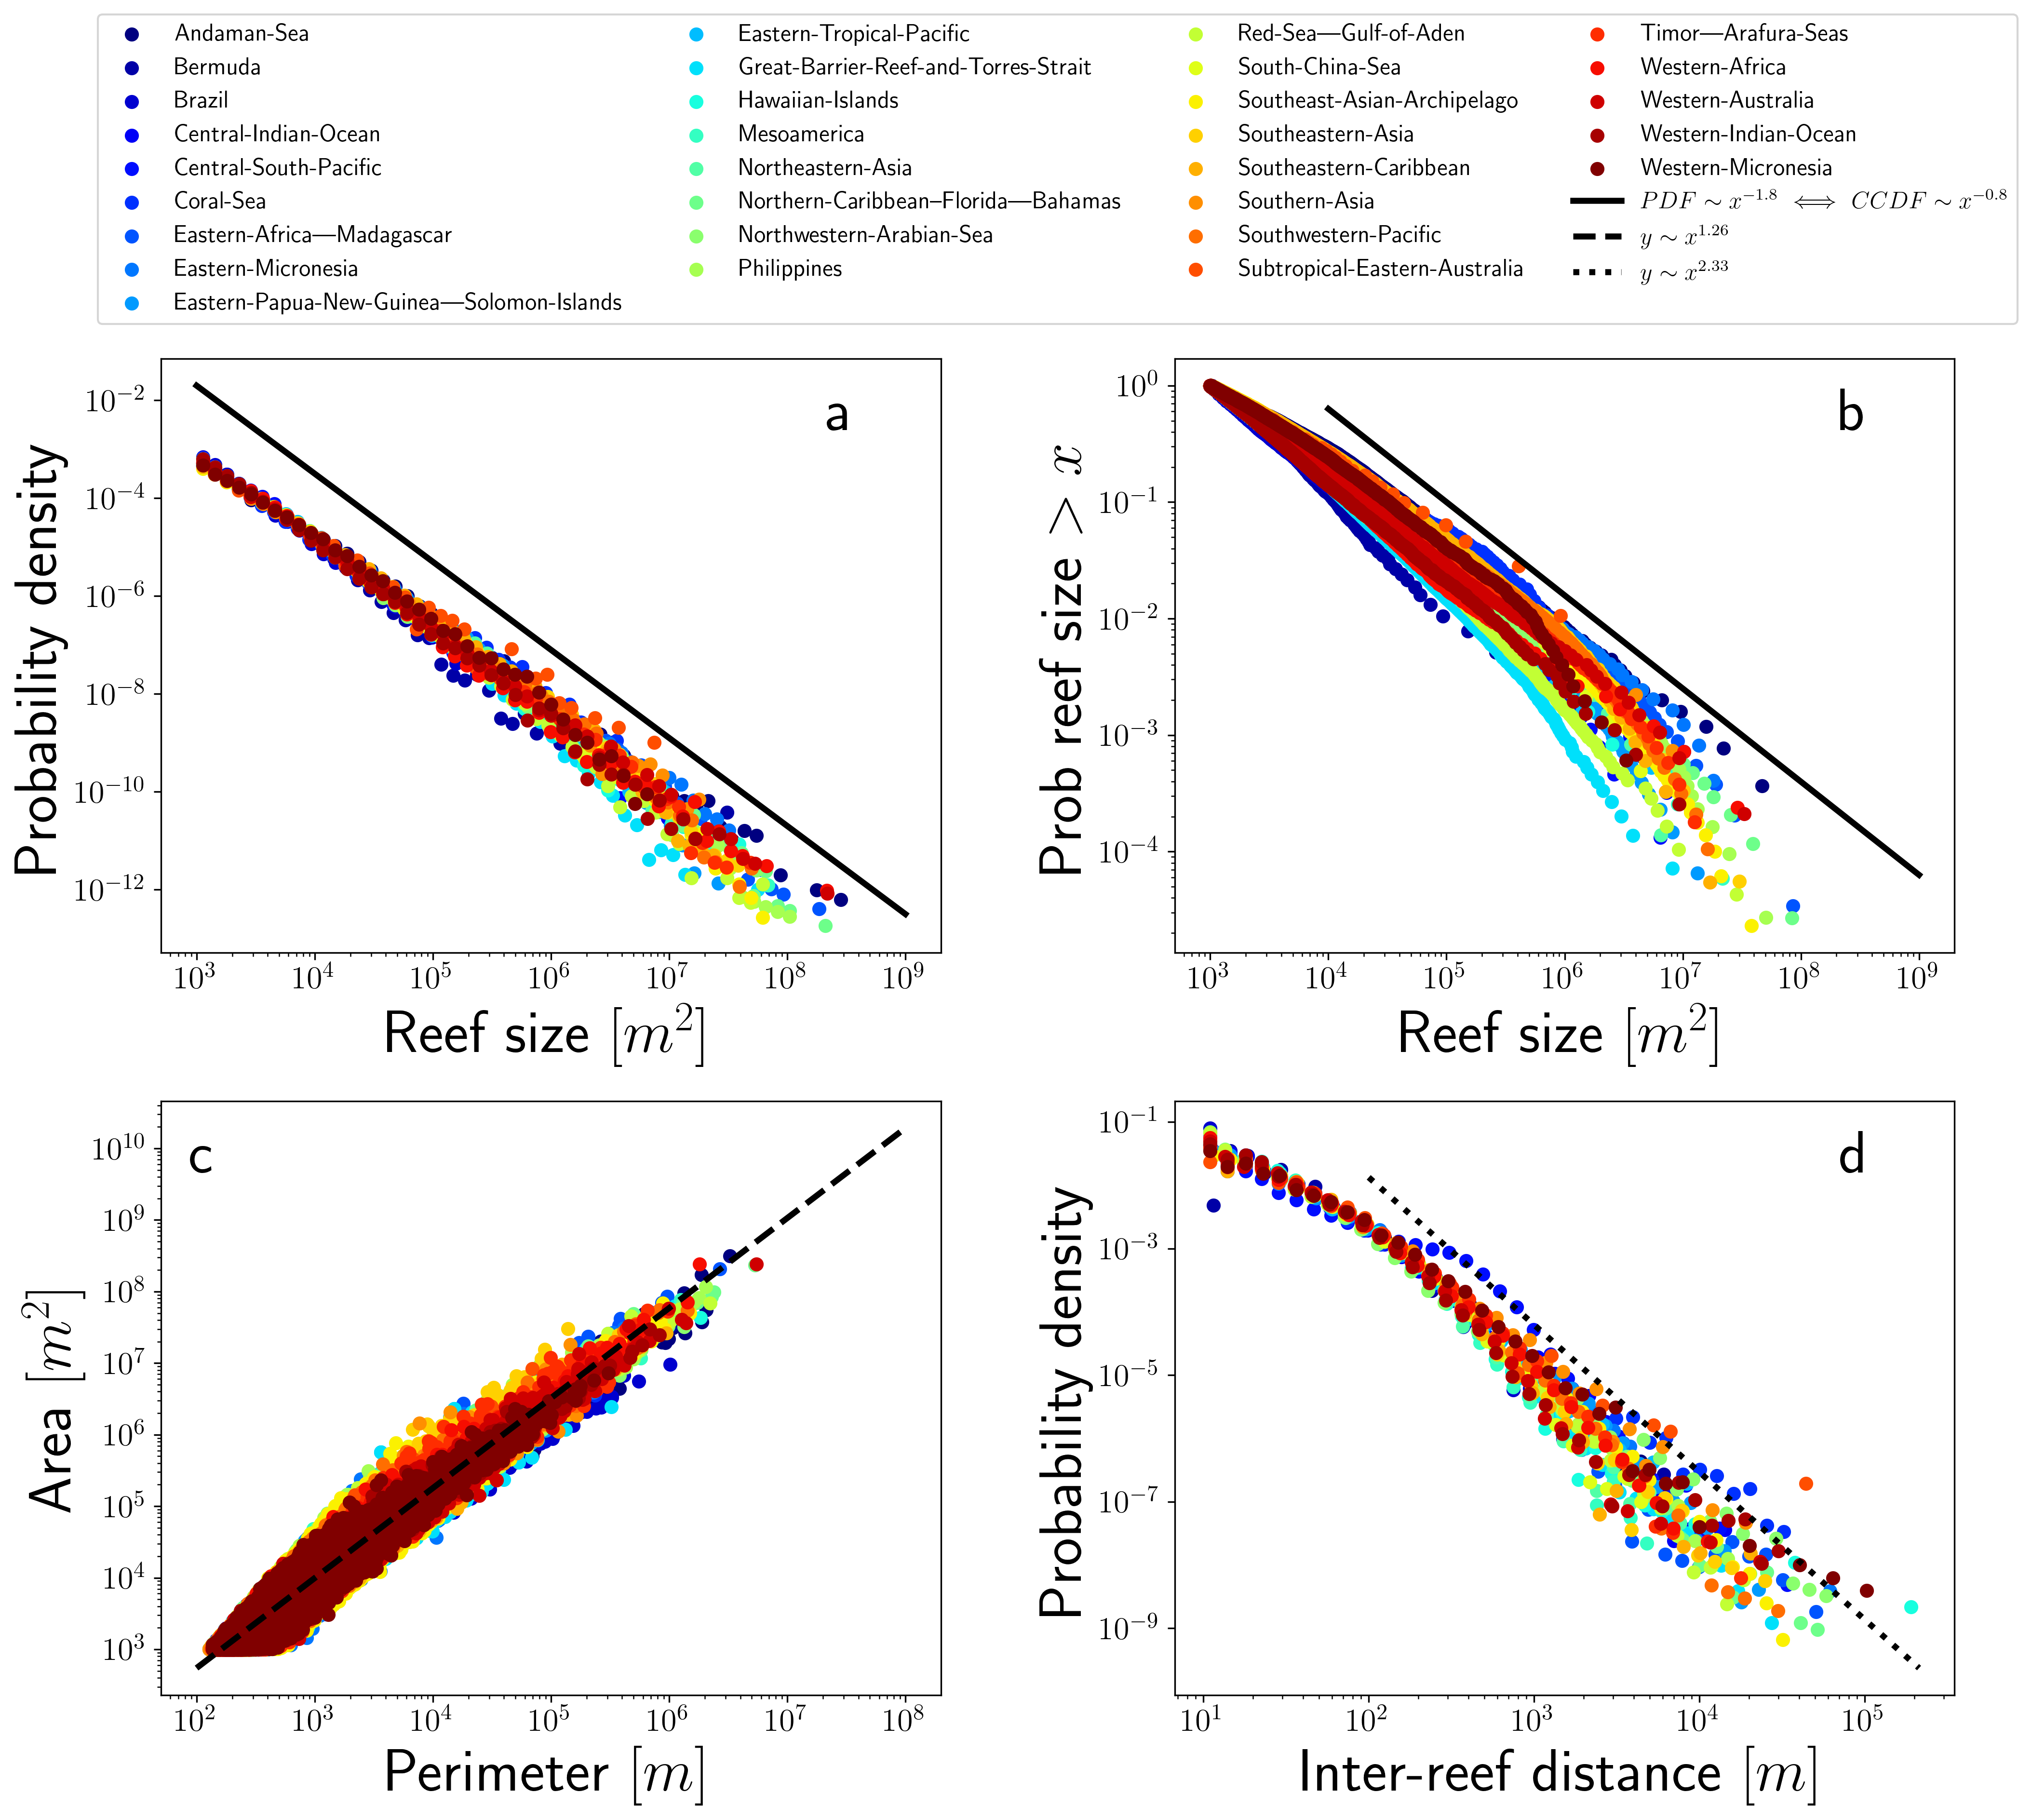
\includegraphics[width=\textwidth]{Figures/general_analysis.png}
    \caption{\textbf{Macroecological patterns of global coral reef size,
            geometry and spacing.} (a) Size distribution. The black line
        corresponds to a
        fitted power-law of exponent $1.8$. (b) Complementary cumulative
        distribution
        function (CCDF) with corresponding exponent of $1.8$. (c)
        Area-Perimeter
        relation. The black dashed line corresponds to a fitted power-law with
        exponent
        $1.23$. (d) Inter-reef distance distribution. The black dotted line
        corresponds
        to a fitted power-law to the distribution tail with a exponent of
        $2.33$.}
    \label{fig:general_analysis}
\end{figure}

The presence of a power-law size distribution also suggests that the object
studied may be fractal in nature \cite{Mori2020, PINTO2014, Seekell2013,
    Sorensen1999, Vidondo1997}, at least along a certain range. A simple way to
test whether coral reefs are fractals is using the area-perimeter relation
\cite{MAN83, Lovejoy1982}, a method of fractal analysis that characterizes the
complexity of irregular shapes by examining the relationship between their area
and perimeter (see Methods). The scaling of coral reef area to perimeter of all
individual coral reefs also converges into a single power-law with an exponent
of $\alpha=1.2578$ ($95\%$ CI: $1.2573$ to $1.2583$), indicating again a
universal behavior (\cref{fig:general_analysis} c). When the relationship is
fitted for each province independently, we found a mean exponent of
$\left<\alpha\right>=1.2574$ ($95\%$ CI: $1.1757$ to $1.3391$), practically
identical to the general exponent. The exponent for the area-perimeter
relationship is significantly lower than the value of $2$ that would be found
for a smooth euclidean geometry. According to fractal analysis, the fractal
dimensions of the perimeter and area of coral reefs are given by $D_P=1.2950$
and $D_A=1.6289$ (see Methods), respectively, which are clearly different than
the putative euclidean dimensions of $D_P=1$ and $D_A=2$. Taking each province
independently, these fractal dimensions would vary between
$D_P^{\mathrm{max}}=1.3506$, $D_P^{\mathrm{min}}=1.2468$ and
$D_A^{\mathrm{max}}=1.6696$ and $D_A^{\mathrm{min}}=1.5879$ within a 95\%
confidence interval, further ensuring that the obtained fractal dimensions are
significantly different from the euclidean geometry. Coral reefs develop
fractal-like geometries, exhibiting complex, self-similar structures across
different scales. This feature might arise from the complex physical and
ecological processes that shape the distribution and growth of coral reefs.
However, how this occurs remains largely unknown, as we lack mechanistic models
able to generate coral reef landscapes across scales and time that can be
challenged to reproduce these patterns.

The spatial distribution of coral reefs within each province was also
investigated by means of the inter-reef distance, defined as the minimum
distance between a reef and its nearest neighbor. We find a heavy-tailed
relation where the tail conforms to a power-law with an exponent of $2.33$
(\cref{fig:general_analysis} d). This reveals that most of the reefs are close
to each other, while a non-negligible number of them are isolated. This finding
is again mostly independent on the geographic location of the analyzed coral
reefs, arising as a universal property of coral reef provinces.

\subsection{The fractal nature of coral reefs}

We computed the fractal dimension of the area and perimeter of each
individual reef from all provinces using the well-known box-counting algorithm
(see Methods). The mean values for the fractal dimension of the perimeter,
$D_P=1.24$ (95\% CI: 1.13 to 1.35) and the fractal dimension of the area,
$D_A=1.60$ (95\% CI: 1.39 to 1.81), are well defined and consistent with those
obtained from the area-perimeter relationship
(\cref{fig:individual_reef_analysis} a,b). The fractal dimension for the reef
areas is quite stable around the mean, although it increases slightly for large
coral reefs (\cref{fig:individual_reef_analysis} a). On the other hand, the
fractal dimension for the perimeter shows a more pronounced increase as
function of reef size. This indicates that as coral reefs grow, their contour
gets more and more convoluted, increasing its complexity, while its surface
remains geometrically more stable.

To further understand the reef formation process from a geometric
perspective, we computed other shape measurements such as compactness and
elongation indices (see Methods). We observe that the compactness of coral
reefs decreases rapidly with increasing size
(\cref{fig:individual_reef_analysis} c). Two changes of shape are consistent
with this result: transitioning from round to elongated shapes or keeping the
rounded shape while developing holes, reef lagoons, within their surface. These
two processes are not necessarily mutually exclusive, as elongated shapes could
appear from evolution of empty rounded shapes. The results obtained for the
elongation index measurement show that both processes must occur, as reefs
elongation increase with size while showing very high variance. This hypothesis
can be contrasted by examining the different shapes that coral reefs have
formed (\cref{fig:individual_reef_analysis} e).

Altogether, our analysis indicate that coral reefs evolve from simple
rounded filled shapes (high compactness and low elongation index) to more
complex elongated and less compact forms (low compactness and high elongation
index), giving rise to fractal objects with stable surface fractal dimension
and increasing perimeter fractal dimension as they grow
(\cref{fig:individual_reef_analysis} e).

\subsection{Fractality extends up to coral provinces}

The fractal dimension of coral reefs varies across a range of spatial
scales, spanning from individual colonies to entire reef systems
\cite{George2021}. This variability arises from the different physical,
biological, and ecological processes that come into play during the development
of the different structures present at each organization level. The different
coral provinces can be understood as the largest organizational level of these
organisms, and the processes involved in maintaining such big structures should
be different from that of individual reefs, giving rise to a different fractal
dimension.

\begin{figure}[H]
    \centering

    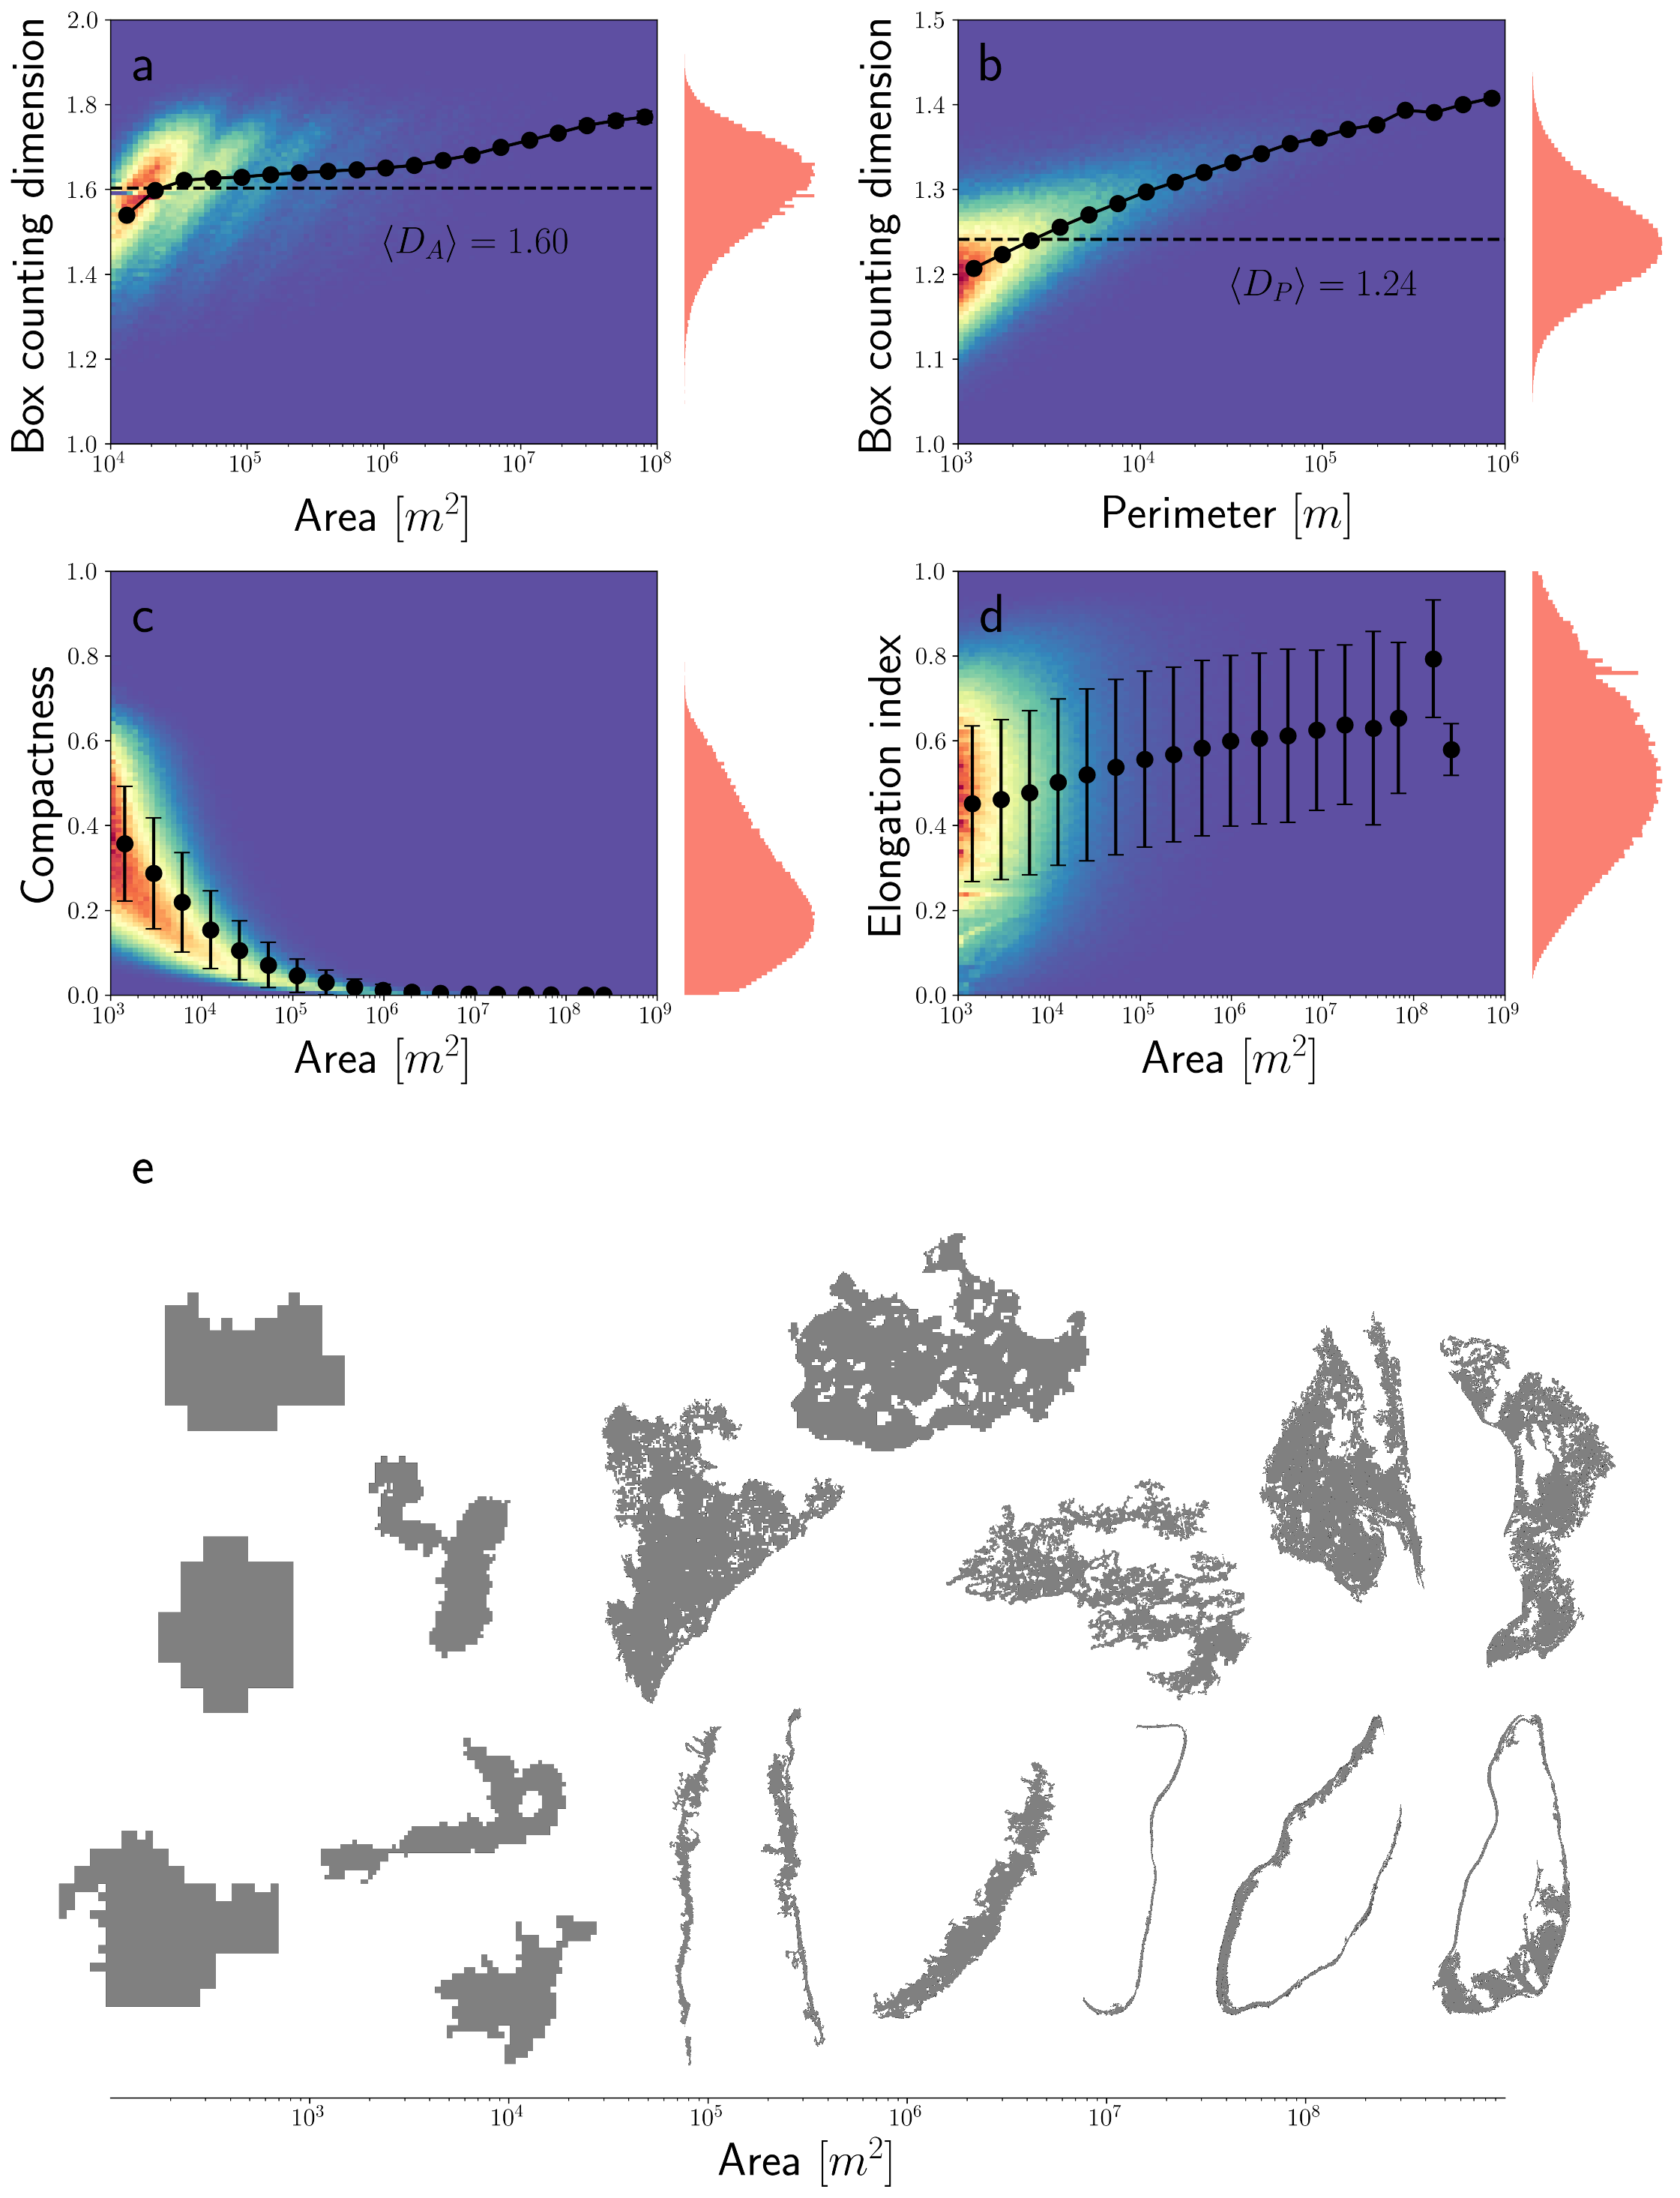
\includegraphics[width=1\textwidth]{Figures/individual_reef_analysis_complete.pdf}
    \caption{\textbf{The fractal nature of global coral reefs.} 2D
        histograms from all shallow-water coral reefs worldwide for: (a) the
        surface
        fractal dimension and area; (b) the perimeter fractal dimension and
        perimeter;
        (c) the compactness and area and (d) the elongation index and area. The
        black
        line corresponds to the mean values of the Y axis measure as function
        of the X
        axis measure. The red histogram corresponds to the distribution of the
        Y axis
        measure. (e) Example of coral reefs shape as function of their
        surface.}
    \label{fig:individual_reef_analysis}
\end{figure}

\begin{figure}[H]
    \centering

    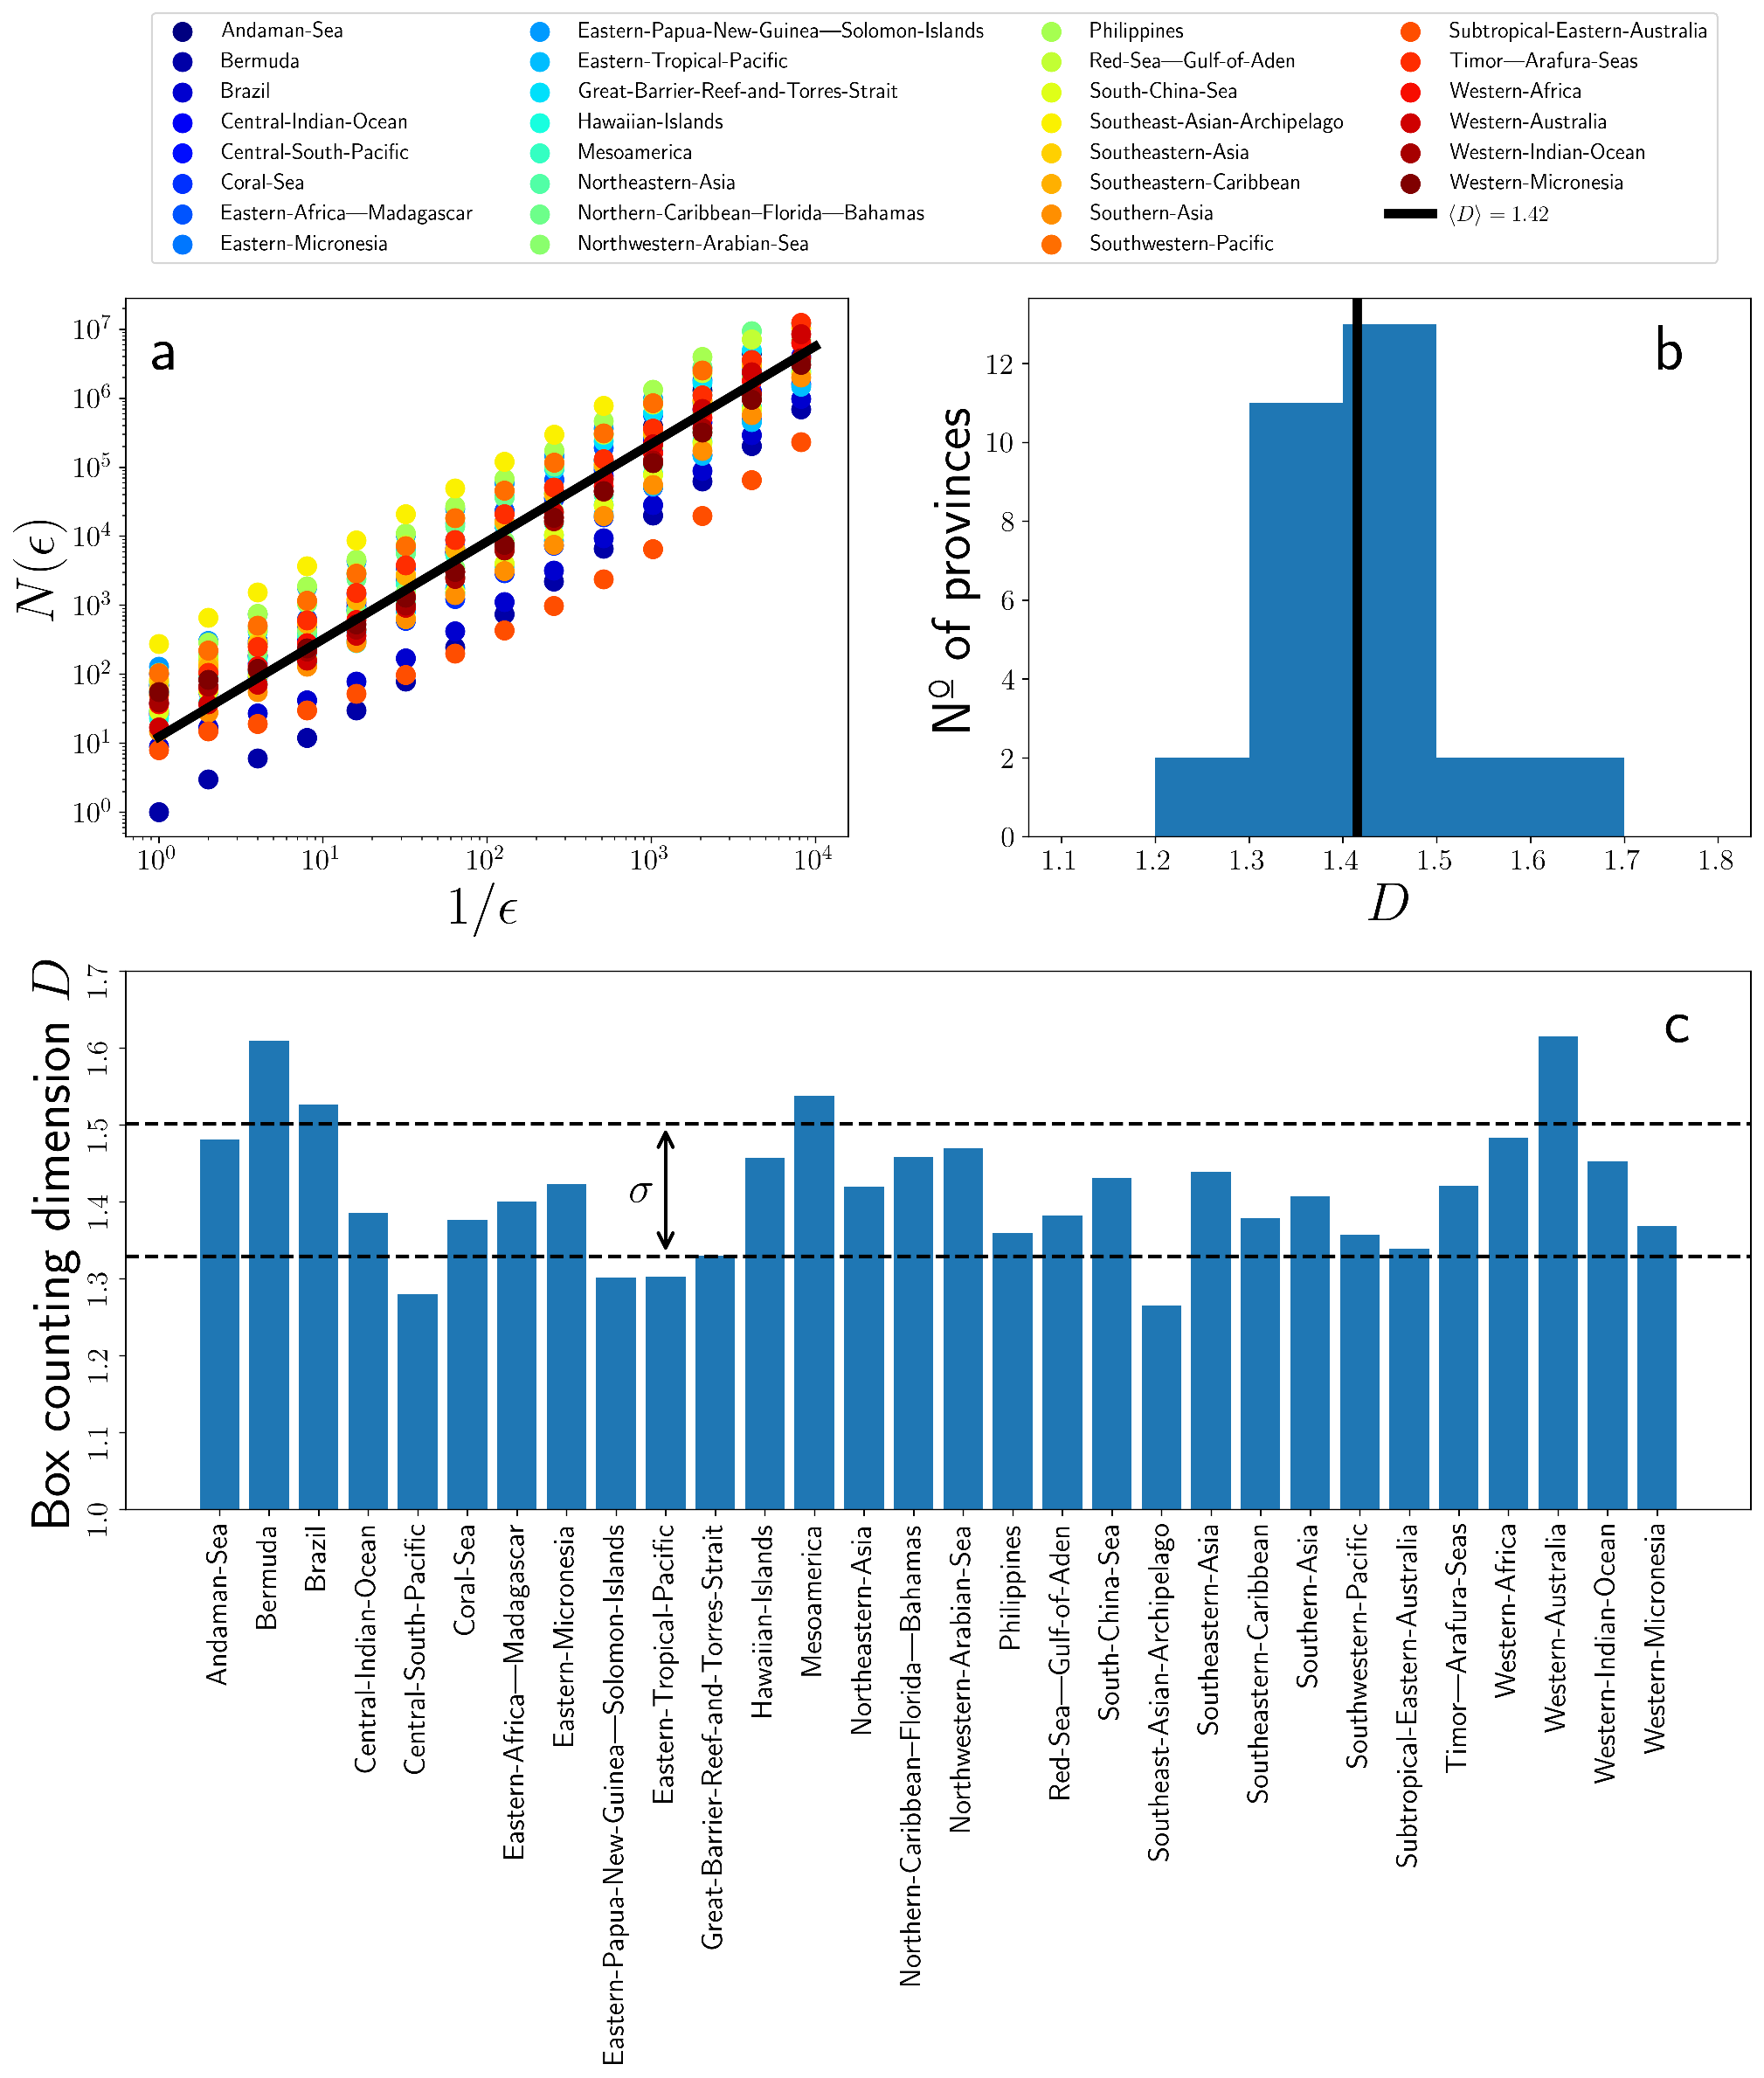
\includegraphics[width=1\textwidth]{Figures/Box_Counting_Dimensions.pdf}
    \caption{Box Counting Dimension of coral reef provinces surface. (a)
        Scaling of the measure (number of boxes of length $\epsilon$,
        $N(\epsilon)$) as
        function of the ruler used (box length $\epsilon$). The slope of the
        fit for
        each province corresponds to its Box-Counting surface fractal
        dimension, $D$.
        (b) Histogram of the obtained Box-Counting fractal dimensions. The
        solid black
        line represents the mean Box-Counting fractal dimension,
        $\left<D\right>$. (c)
        Box-counting surface dimension for each coral province. Black dashed
        lines
        correspond to a 1 $\sigma$ deviation from the mean.}
    \label{fig:Box_Counting_Dimension}
\end{figure}

To investigate this hypothesis, we computed the surface fractal dimension
for each coral province as a whole using the well-known box-counting algorithm
(Methods, \cref{fig:Box_Counting_SI}). We found a mean fractal dimension
of
$\left<D\right>=1.42$ (95\% CI: 1.24 to 1.59), consistent across the different
coral provinces assuming a normal distribution
(\cref{fig:Box_Counting_Dimension}). The fractal dimension of coral reef
landscapes is similar to those expected from sizes expanding along a Fibonacci
series, which yield a fractal dimension of 1.44 \cite{Sorensen1998}. This
suggests, again, that coral reefs are self-organized systems that exhibit
similar patterns of complexity and irregularity at different scales, and that
the fractality is an intrinsic property of coral reefs that likely arise from
the underlying biological, physical, and ecological processes involved in their
growth dynamics.

\section{Discussion}

Coral reefs self-organize to form macroecological patterns that are largely
independent of the geographical location of the reefs, suggesting that the
specific physical conditions to which each coral province is subject have
little influence on the development of these scaling laws. Coral reef
geometries conform fractal structures that follow a power-law size
distribution, with many reefs close to each other while others are completely
isolated across coral reef provinces. Overall, our findings provide strong
evidence that the power-law size distribution of coral reefs and their fractal
geometries are fundamental features of these ecosystems, which reflect the
underlying ecological and physical processes that shape them across scales.
Furthermore, because the exponent of the power-law size distribution and the
fractal dimensions are consistent across different regions, these features are
not only fundamental, but universal laws reflecting coral reef growth
processes.

These universal scaling properties must be used to challenge mechanistic
models aimed at reflecting coral reef growth, which hitherto lacked such
constraints, both as individual reefs as well as coral reef provinces. For
example, at the scale of coral reef province, the characteristic spacing
(inter-reef distance distribution) likely influences the interaction between
coral reefs, hydrodynamic flows, and the dynamics of the limiting nutrients
transported to support photosynthesis and calcification, further constrained by
sea level change and available vertical accommodation space \cite{Nakamura2007,
    Mistr2003, Bosscher1992}. Realistic models of coral reef growth and
dynamics
should be able to reproduce the universal features described here, such as the
power law in coral reef size distribution, the fractal geometries and the
changes in reef shape with size.

Power-law distributions have been also found in many natural systems
\cite{SOLE1995, west2000scaling, Brown2002, Chave2003, Marquet2005,
    Corral2019}.
Different mechanisms can produce such emergent power-laws
\cite{Markovic2014}: Self-Organized Criticality, in which the system evolves
naturally towards a critical state \cite{Per1988}; Highly Optimized Tolerance,
in which the systems evolves following a trade-off between yield, cost of
resources and tolerance to risk \cite{Carlson1999,Carlson2000}, or correlated
noise models, in which external drives and internal dynamics compete on similar
time scales, yielding a non-critical steady state characterized by heavy-tailed
distributions \cite{Newman1996}. Ecological power-laws can arise through a
combination of several ecological and physical processes, including competition
for resources, random disturbances leading to failure or loss. In
\cite{Scanlon2007, Kefi2007} it was shown that the emergence of power-laws in
vegetation patterns requires the interplay between global competitive and
locally facilitative interactions \cite{Scanlon2007, Kefi2007}. These power-law
distributions are different than those obtained in classical critical systems,
where power laws occur exclusively at the transition point
\cite{Wilson1979,Binney1995}. Actually, the ecological power-law reported in
\cite{Kefi2007} only occurs far enough from the (true) critical transition to
extinction. It has been conjectured that living systems exhibiting this
behavior could draw important functional advantages from operating close to an
emergent critical point, namely an optimal balance between robustness and
flexibility \cite{Munoz2018}. In the case of corals, this could reflect a
balance among self-organization dynamics driven by competition for space and
resources with other species, environmental factors like ocean currents and
water quality, predation interactions within the reef ecosystem and local
facilitative interactions, such as energy disspiation. The combination of these
mechanisms should be explored in developing models of coral reef formation.

Fractal models have been also used to investigate universal principles that
govern the structure and dynamics of complex ecological systems
\cite{Brown2002}, such as the geometry of benthic ecosystems or power-law
scaling \cite{Schmid1999}. In coral reef ecosystems, fractal geometry might
emerge as an efficient structure for nutrient acquisition \cite{Sous2020}. The
fact that $D_P>1$ implies that the reef contour is highly convoluted, while
$D_A<2$ is the result of the development of multiples holes in the reef
surface. The combination of these mechanisms maximizes the chance that coral
individuals living at the reef surface are in contact with an external flow,
thus being able to obtain nutrients. According to \cite{George2021}, coral
colonies with a larger space-filling surface and smaller perimeters increase
energy gain while reducing the exposure to competitors. A similar argument
could apply in the case of coral reefs, which can be included in modeling
approaches.

The shape of coral reefs varies with size, and thereby during growth, from
more compact, circular structures at small size, observed at the mean area of
3.32 ha, to increasingly elongated structures, which may break the closed shape
to form long, linear, fringing reefs. The change in geometry from circular to
fringing has been postulated to result mostly from reduced accommodation space
as coral reefs grow, and the interaction with sea level \cite{Kennedy2002}, but
has also been explained as resulting from the interaction between reefs and
nutrients transported along hydrodynamic flows from a prevalent direction
\cite{Mistr2003}. Reefs inside reef structures can be also observed, suggesting
that as coral reefs expand in size, smaller reefs appear inside them, starting
as compact coral heads to then develop empty inner spaces. Overall, this
phenomenology suggests that a Turing instability
\cite{turing1952chemical,CrossGreensidebook} might be present, which indeed has
been previously suggested \cite{Mistr2003}, arising due to the interplay
between diffusion of nutrient species and nutrient uptake and recycling
processes within reefs. However the Turing mechanism would yield a normal
distribution of inter-reef distances, not compatible with the heavy-tailed
inter-reef distance distribution found in this study neither with the obtained
power-law scaling.

Overall, our findings have important implications for understanding of the
structure and function of coral reefs, as well as for their conservation and
management. The macroecological characterization of universal laws in the
geometry of coral reefs, along with the dataset of unique coral reefs globally,
which are reported here for the first time, should help design effective coral
reef restoration projects as well as optimize and quantify the effort and
resources required.

\section{Methods}

\subsection{Global coral reef data}

Global-scale coral reef benthic data were obtained from the Allen Coral
Atlas (ACA) \cite{allen-coral-atlas}, a publicly available dataset of
high-resolution satellite imagery and machine learning-based coral reef
classifications. We downloaded the data from the ACA website, which is already
divided into the different coral reef provinces. The downloaded dataset
consists of GeoJSON files for each coral province with several Polygons and
Multiploygons forming the different benthic classes, from which we selected the
``coral/algae'' class (see \cite{allen-coral-atlas}). Despite the data is
already provided in vector format, the reefs are not identified as individual
entities, i.e. a single reef can be formed by many polygons or multipolygon
objects. Thus, we processed the dataset with the methods explained below to
obtain a representation of individual reefs.

\subsection{Coral reefs as clusters of connected coral/algae class polygons}

A label assignment algorithm was developed to identify the different
independent (not connected) components forming the coral reefs. Basically, we
followed an iterative process in which connected components were assigned the
same label, thus being identified as forming the same component. Polygons were
considered to be connected if they intersected. To efficiently compute the
intersections among polygons we used the Sort-Tile-Recursive algorithm
\cite{STRtree} implemented in Python Shapely library \cite{shapely}. The
implementation of the algorithm can be found in the Preprocessing.py module at
\cite{CODE_corals}.

Coral reefs of less than $10^3\,\textrm{m}^2$ were considered as possible
noise in the dataset, and thus disregarded. We made this choice based in the
fact that the ACA is obtained from satellite imagery of about $3\,\textrm{m}$
resolution. Thus, coral reefs of less than this area would represent less than
$100$ pixels.

\subsection{Coral reefs area, perimeter and inter-reef distance}

We computed coral reef area and perimeter using the
\textit{geopandas.GeoSeries.area} and \textit{geopandas.GeoSeries.length}
methods in geopandas Python's library \cite{Geopandas}. For each coral reef, we
defined the inter-reef distance as the distance to its nearest neighbor. Thus,
the inter-reef distance distribution is obtained after obtaining the nearest
neighbor to each reef and computing that distance. To make this computation
efficient, we used the Sort-Tile-Recursive algorithm \cite{STRtree} implemented
in Python Shapely library \cite{shapely}. The implementation of the algorithm
can be found in \cite{CODE_corals}.

We note that our estimates of the total area for each coral reef provinces
(\cref{tab:Province statistics}) slightly differ from that directly provided
by the ACA because we removed ``reefs'' smaller than $10^3\, \textrm{m}^2$. Of
course, if the area is computed before this data cleaning step the results are
identical.

\subsection{Coral reef size distribution}

We fitted the coral reef size data using the powerlaw package in Python
\cite{powerlaw, Clauset2009}. We performed goodness-of-fit tests using a range
of alternative distribution models, including log-normal, exponential, and
stretched exponential distributions. We found that the power-law distribution
(including its truncated form) provided a significantly better fit to the data
than any of the alternative models with $x_{\textrm{min}}$ ranging from
$10^3\,\textrm{m}^2$ to $10^4\,\textrm{m}^2$
(\cref{tab:dist_comparison,tab:fit_results}).

\subsection{Fractal dimensions from area-perimeter relation}

The area of regular objects such as squares or circles scale as the square
of the perimeter $A\sim P^2$, while the area of irregular fractal objects scale
more generally as $A\sim P^{\sigma}$, where $\sigma=D_A/D_P$ with $D_A$ and
$D_P$ being the fractal dimension of the area and the perimeter, respectively
\cite{MAN83, CHEN2013}. These fractals dimensions can be easily computed from
the area-perimeter scaling exponent, $\sigma$, as $D_P=(2+\sigma)/2\sigma$ and
$D_A=(2+\sigma)/2$ \cite{CHEN2013}.

\subsection{Box-Counting fractal dimension}

We computed the Box-Counting fractal dimension of all mapped areas
following a box-counting algorithm \cite{MAN83}. Briefly, the method computes
the number of boxes of length $\epsilon$, $N(\epsilon)$, needed to cover the
underlying object. Then, the fractal dimension is simply defined as,
\begin{equation}
    D=\lim_{\epsilon\to 0}\frac{\ln{N(\epsilon)}}{\ln{1/\epsilon}} \ .
\end{equation}
In practice, the mathematical limit $\epsilon\to 0$ is unreachable and the
fractal dimension is computed from the slope obtained in the plot of $\ln
    N(\epsilon)$ versus $\ln(1/\epsilon)$. To efficiently compute the number of
overlapping boxes we used the Sort-Tile-Recursive algorithm \cite{STRtree}
implemented in Python Shapely library \cite{shapely}. The implementation of the
algorithm can be found in \cite{CODE_corals}.

\subsection{Compactness and elongation index}

The compactness measurement is defined as the isoperimetric quotient,
\begin{equation}
    C=\frac{4\pi A}{P^2} \ ,
\end{equation}
where $A$ and $P$ are the area and perimeter of the object under study,
respectively.

The elongation index is defined as the Flaherty \& Crumplin (1992)
length-width measure, stated as measure LW\_7 in \cite{Altman1998} and
implemented in PySAL Python's library \cite{pysal2007}.